\documentclass[11pt,onesided]{memoir}

\def\watermarkloaded{0}

\def\Title{ally}
\def\Subtitle{}
\def\FullTitle{\Title}
\def\AuthorFirst{Madison}
\def\AuthorLast{Scott-Clary}
\def\AuthorFull{\AuthorFirst\ \AuthorLast}

\def\Edition{First}
\def\EditionsList{10 9 8 7 6 5 4 3 2 1}
\def\Year{2017}

\def\ISBN{XXX-X-XXXXXX-XX-X}

\newenvironment{ally}{
\noindent\ignorespaces
\begin{quotation}
    \allyFont\itshape
    \noindent}{
\end{quotation}\ignorespacesafterend }

\input{includes/draft}
\input{includes/frame}
\input{includes/packages}
\input{includes/geometry}
\input{includes/toc}
%%% Font
% Uncomment and modify to your font specs

\usepackage{fontspec}
\setmainfont{Gentium Book Basic}
\newfontfamily\allyFont{Merriweather Sans}[Scale=0.9,Color=444444FF,Ligatures=TeX]
\newfontfamily\TitleFamily{Inknut Antiqua}
\newfontface\TitleFont{Inknut Antiqua}
% \newfontfamily\DisplayFamily{Playfair Display}
% \newfontface\DisplayFont{Playfair Display}

\input{includes/pagelayout}
\input{includes/title}
\input{includes/secdiv}
\input{includes/hyphenation}

\begin{document}
  \frontmatter

  \includepdf{cover.pdf}
  \thispagestyle{empty}
\null
\vfill
\begin{flushright}
  \allyFont\Large\FullTitle
\end{flushright}
\vfill
\cleardoublepage


  \pagestyle{plain}

  \doublespacing

  \null
  \vfill
  \begin{flushright}
    {\fontspec{Merriweather Sans}[Scale=1.5,Color=444444FF]\Huge ally}

    \vfill
    
    {\fontspec{Merriweather Sans}[Scale=1.5,Color=555555FF]\normalsize from start to finish}
    \vfill
    {\Huge Madison Scott-Clary}
  \end{flushright}
  % \vfill
  \thispagestyle{empty}

  \newpage

  \singlespacing
\thispagestyle{empty}
\null
\vfill
{\parindent0pt
No part of this work may be reproduced or transmitted in any form or by any means, electronic or mechanical, including by photocopying or recording, or by any information storage or retrieval system without the proper written permission of the copyright owner unless such copying is expressly permitted by federal copyright law.Permission must be obtained by the author. Address requests for permission to make copies of material here to the email address makyo@drab-makyo.com

\vspace{1ex}

ISBN: \ISBN

\vspace{1ex}

\textsc{\FullTitle}

\vspace{1ex}

Copyright \copyright\ \Year

\vspace{1ex}

\Edition\ Edition, \Year. All rights reserved.

\vspace{1ex}

\vspace{1ex}

\vspace{1ex}

Printed in the United States of America\\
\EditionsList
}%\parindent0pt

\clearpage


  % \tableofcontents*
  \newpage
  \null
  \thispagestyle{empty}
  \cleardoublepage

  \onehalfspacing

  % \input{content/preface}
  \null
  \vfill
  \begin{center}
    How many layers of remove is enough?

    \vfill

    We ask how, because the question of why must ask itself.
  \end{center}
  \vfill

  \mainmatter

  \pagestyle{ourbook}
  \columnratio{0.65}
  \setlength\columnsep{20pt}
  %\twosided
  \backgroundcolor{c[1]}[HTML]{eeddff}
  \backgroundcolor{C[1](0.5\columnsep,10000pt)(10000pt,10000pt)}[HTML]{eeddff}
  What if I tried to write a memoir?

Like.

It doesn't need to be totally true, and maybe some stuff gets pretty floaty, and maybe some stuff winds up as poetry, and maybe some of it is ergodic with scans of notes or bits of other projects scattered throughout, and maybe I just own the hypertextuality of the medium, but it's generally autobiographical.

That might be neat

\ally{Who are you kidding?}

Myself, I guess.

\ally{Well, have at it, then.}

\newpage

  \backgroundcolor{c[1]}[HTML]{ffddee}
  \backgroundcolor{C[1](0.5\columnsep,10000pt)(10000pt,10000pt)}[HTML]{ffddee}
  \chapter*{\allyId}

\label{site}

\begin{paracol}{2}
\begin{leftcolumn}
We promise ourselves that we live our memories in a linear fashion. And who knows, perhaps we do.

What we emphatically do not do is remember our lives in linear fashion. \allyWord\ began as an interactive project specifically to explore this aspect. The goal was to use the concept of interlinked pages to represent the way that one memory can be interlinked to another, and another, and so on.

\begin{ally}
  And dreadfully distinct within the dark, a tall white fountain played?
\end{ally}
Something like that.

And here, we lean on a very specific deinition of hypertext. Hypertext is used to imply that some portion of a document can link to another portion of a document. This linking goes beyond simply the links that one clicks, as it can mean inclusions, such as when an image is included on a page full of text. It can, indeed, mean a link that leads from one page to the next, but what means `next' here? Does it mean moving on to the next page in a series of pages, or does it mean moving from one section of the site to another? Perhaps it means moving from this site to the next.

\end{leftcolumn}
\begin{rightcolumn*}
\newpage
\section*{Hypertext types}
\begin{labeling}{Arborescent}
  \item[Axial] A set of linked documents that travels down a single axis, from start to finish.
  \item[Arborescent] A set of linked documents with a central axis, of of which may sprout other documents (which may in turn be axial or arborescent hypertexts).
  \item[Networked] A set of linked documents with no discernable axis. No start or finish, no direction to travel in.
\end{labeling}
\end{rightcolumn*}
\begin{leftcolumn}

With \allyId, this became a core component of exploring memory. It means something different to wind one's way down the singular path a memory treads than it does to jump the track onto something wholly different. The central axis of the story is the death of Matthew as told through conversations with--

\begin{ally}
  Me!
\end{ally}
--with an imaginary alter-ego who, by virtue of that `ego', knows all the same things I do.

\begin{ally}
  Or more.
\end{ally}
Perhaps, yes.

As a memory would be touched upon, it would spark a new branch of exploration that would proceed in much the same way. This is why the project is described as ``arborescent'': there is a central trunk with a defined beginning at the root, and from there, it blossoms up and out.

Or, it turns out, down and out.
\newpage

\end{leftcolumn}
\begin{rightcolumn*}
\begin{verse}
\begin{spacing}{-10}
{\MonoFont
.\\
├── about.md\\
├── ally\\
│   ├── 001.md\\
│   ├── 002.md\\
│   ├── ...\\
│   └── \_index.md\\
├── birds\\
│   ├── 01.md\\
│   ├── 02.md\\
│   ├── ...\\
│   └── \_index.md\\
├── burnout\\
│   ├── 01.md\\
│   ├── 02.md\\
│   ├── ...\\
│   └── \_index.md\\
├── dad\\
│   ├── 001.md\\
│   ├── 002.md\\
│   ├── ...\\
│   ├── as\\
│   │   └── a\\
│   │       └── person\\
│   │           ├── 001.md\\
│   │           ├── 002.md\\
│   │           ├── 003.md\\
│   │           ├── 004.md\\
│   │           ├── 005.md\\
│   │           └── \_index.md\\
│   └── \_index.md\\
└── ...
}
\end{spacing}
\end{verse}

\end{rightcolumn*}
\begin{leftcolumn}
\noindent While working on \allyId, Each page was kept in a single Markdown file, and each exploring branch was kept in a folder. Thus, we wind up with a file structure akin to what we see on the right.

\begin{ally}
  Never content to condense your thoughts into something simple and easy to read, were you?
\end{ally}
To your scattered files go, I suppose.

Do keep in mind that this is a website, however. This directory, these filenames, this structure all play a role in how the whole project works. These whole tree of files are in the \texttt{content} directory of a Hugo project. Hugo is a program which knows how to take these Markdown files and turn them into HTML files while following a simple set of rules.

In each of those \texttt{\_index.md} files, one will usually find nothing. That is, in terms of content, for at the top of each file comes a header which describes some of those rules. For instance, in some directories, we want the background to be a certain color, or perhaps we want there to be a link down at the bottom saying ``back to where we left off''.

\begin{ally}
  There is no going, and there is no back.
\end{ally}
We can always pretend.

Another rule that is stated in these files is that they are intended to list the pages in that directory. Usually, this is done on a blog page where you might see the titles and first paragraphs of ten blog entries in a list, each with a ``read more'' link, followed at the bottom by a list of `pages of results'. In my case, though, I set Hugo up so that, when it listed all of the `posts', it would only do one per page, and instead of showing only the first paragraph, it would show the whole page. This essentially made it work as a book would: you simply turn the page when you're done reading. My \texttt{list.html} file for this `serial' layout loops over the pages in the directory as follows:

\begin{verbatim}
{{ $paginator := .Paginate .Pages.ByWeight 1 }}
{{ $content := .Content }}
{{ range $paginator.Pages.ByWeight }}
...
\end{verbatim}

With this theme in place and with the files all in the right orders (each with a \texttt{weight} key in their own headers), Hugo will build the site as it stands.

\begin{ally}
  Oh, but there's more to it than that.
\end{ally}
Of course.

\newpage
\end{leftcolumn}
\begin{rightcolumn*}
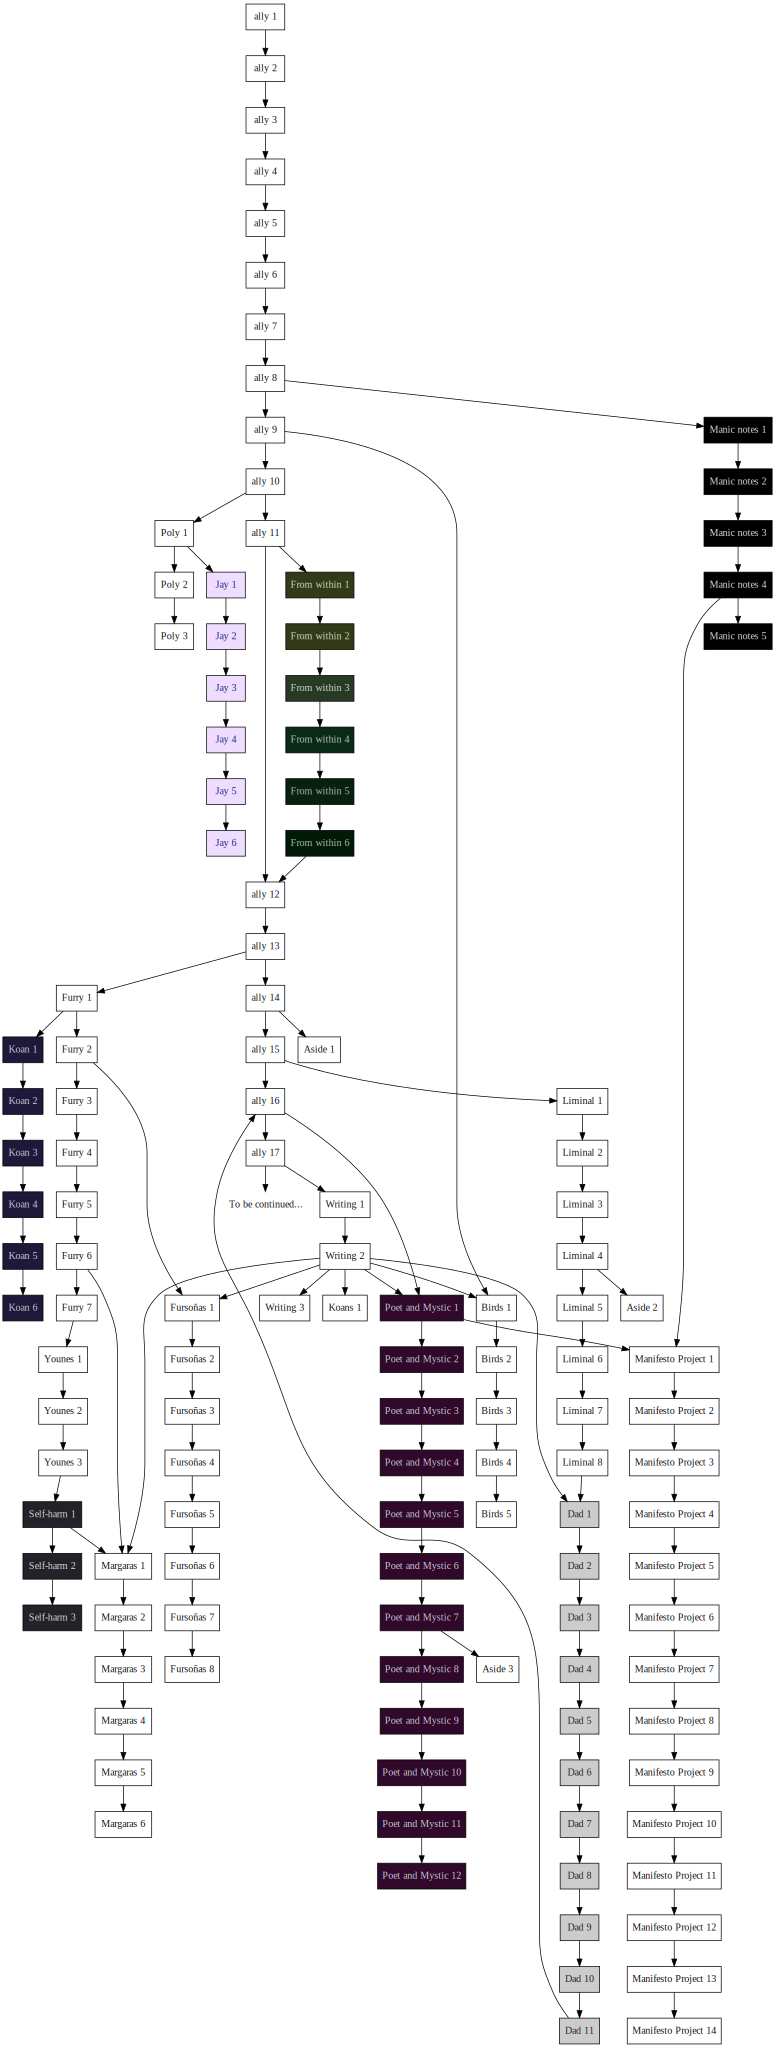
\includegraphics[width=2.5in]{assets/map.png}
\end{rightcolumn*}
\begin{leftcolumn}

\noindent Early on in \allyId's life, I decided that there needed to be a map of the site. A literal map, too. No carefully broken down list of links for you to click on, but something more clearly representing the paths one takes through memory.

\begin{ally}
  Your ``Catastrophically Maddy'' counter is ticking up.
\end{ally}
Did you expect anything less?

\begin{ally}
  I suppose not. Carry on.
\end{ally}
Score one for Maddy.

So, even thought it takes a bit of work by hand everytime I add a page, I decided that it would be worth it to construct a graph that showed the arborescent nature of the project. I was tempted at one point to do the whole thing in Javascript using SVG so that it would track your movement through the pages, but even that was too much for me.

\begin{ally}
  Wonder of wonders.
\end{ally}
So instead, I leveraged existing tools--

\begin{ally}
  Gag.
\end{ally}
Right, sorry. So instead, I decided to use what I already had installed, which meant dusting off my knowledge of Graphviz.

In my \texttt{assets} folder lives a \texttt{map.dot} file which contains a node for every page and the edges that connect them. It's easy to add to; every time I add a new branch, I list every page inside of it along with its URL, and then draw all of the links that connect those pages together. At the bottom, there is the links from the trunk (or parent branch) to the branches.

\begin{verbatim}
digraph Map {
    node[group="dad",
         style="filled",
         fillcolor="#cccccc",
         fontcolor="#222222"]
    "Dad 1" [href="/dad"]
    "Dad 2" [href="/dad/2"]
    "Dad 3" [href="/dad/3"]
    "Dad 4" [href="/dad/4"]
    "Dad 5" [href="/dad/5"]
    "Dad 6" [href="/dad/6"]
    "Dad 7" [href="/dad/7"]
    "Dad 8" [href="/dad/8"]
    "Dad 9" [href="/dad/9"]
    "Dad 10" [href="/dad/10"]
    "Dad 11" [href="/dad/11"]
    "Dad 1" -> "Dad 2" -> "Dad 3" -> "Dad 4" -> "Dad 5" ->
    "Dad 6" -> "Dad 7" -> "Dad 8" -> "Dad 9" -> "Dad 10" ->
    "Dad 11"
\end{verbatim}

And so on, until:

\begin{verbatim}
    "ally 29" -> "Burnout 1"
    "As a person 5" -> "ally 16"
    "From within 6" -> "ally 12"
    "Younes 3" -> "Self-harm 1"
    "Furry 1" -> "Koan 1"
    "Jay 3" -> "Dreams 1"
    "Liminal 8" -> "Dad 1"
}
\end{verbatim}
\newpage

While the whole file is much, much larger than just this, it is really no more complicated\footnote{Except\ldots{} --- page \pageref{branchdir}}. I rarely go back and change orders, and almost never tack a branch onto the trunk in a different place, so I just trace the lines once and let Graphviz sort the rest out.

Once I've updated the Dot file with the new pages, I type \texttt{make}, which, on seeing that the file has changed, runs \texttt{dot -Tsvg map.dot -omap.svg}, which generages the image itself.

The cool part about SVG is that it renders in the browser just as well as HTML, including with clickable links, so I get a \emph{navigable} sitemap for free. All I need to do is copy and paste the contents of that \texttt{map.svg} file into the proper place in the site\footnote{\ldots{}sorta --- page \pageref{svgfont}}. 

\newpage

We have our content, we have our map, now we just need a way to get it up on the web so that others can see it, right?

\begin{ally}
  A question like that never has an easy answer.
\end{ally}
Correct.

Hugo generates a set of folders filled with HTML files and static assets. It's no good on my machine, since that'd mean that I'm the only one that can see it. I could FTP the project up to a server and drop it where everyone could see that but\ldots{}you know, now that I think about it, I can't remember the last time I used FTP.

Better, instead to just have another tool do it for me. Two other tools, actually.

\begin{ally}
  You know, if you are trying to sell this as an easy way to approach a project, I don't know that you are succeeding.
\end{ally}
This is fair. One of the reasons it feels easy to me is that I was already running several other projects using the same technology. The reasons those work so well for me are closely tied with how I run my writing setup, and how I use my writing setup is closely tied with how I program.

It makes sense for me to have a system that relies on convention over configuration, given how many software projects have worked that way. It makes sense for me to have a system that relies on publishing stories in files rather than database entries as I might with Wordpress or Ghost, given how much of my life is spent tooling around with other files. I'm hardly recommending this as a path forward. There are doubtless easier ways, regardless of how well this worked for me.

\begin{ally}
  Right.
\end{ally}
Right.

So, given this Hugo site, the best way for me to work with deploying it uses a pair of tools: Github, which allows me to keep the entire site in a version-controlled repository synced remotely, and Netlify which will automatically build and serve static sites such as this one.
\end{leftcolumn}
\begin{rightcolumn*}
\includegraphics[width=2in]{assets/workflow.png}
\end{rightcolumn*}
\begin{leftcolumn}

When I get an idea for a ``sidequest'' to work on with \allyWord, I create a branch away from the \texttt{master} branch --- `branch' both in terms of git as well as in terms of hypertext, here --- and work there. When I push that branch up to Github and create a pull request, Netlify sees this and automatically creates a deploy preview which I can share with those Patrons who get early access. When I click the big grean ``merge'' button on github, Netlify then builds the main site which everyone can see
\newpage
\end{leftcolumn}
\end{paracol}

  \backgroundcolor{c[1]}[HTML]{ddffee}
  \backgroundcolor{C[1](0.5\columnsep,10000pt)(10000pt,10000pt)}[HTML]{ddffee}
  \begin{quote}
Do you remember when you met me?
\end{quote}

When I met you? I don't remember it so much as a meeting as you were just already there.

\begin{quote}
I was, yes.
\end{quote}

After high school, then. That's when you showed up. That's when life began. That's when I started thinking of myself as a person. That's when I started thinking of others as people, with their own motivations, their own desires, their own incentives and failings.

\begin{quote}
And you made it through.
\end{quote}

After a fashion.

\begin{quote}
You're here, now. You made it through.
\end{quote}

She never wanted to be What she became; The irony of which Is not lost on her.

\begin{quote}
Touching.
\end{quote}

Hey now, don't be rude. Aren't you supposed to be my ally?

\begin{quote}
I \textbf{am} your ally. I'm just not your friend.
\end{quote}

Fair enough.

So you showed up after high school. You showed up after life slid sideways through puberty. I went digging, you know. To find this out.

\begin{quote}
Oh?
\end{quote}

Yeah. June 2004. There you are. I say,

\begin{verbatim}
The navy blue I've been seeing at waist level in front of me and to my left is contentment. I'm not entirely sure that it being omnipresent is a good thing, however, considering the colors it's mixed with. Am I really content with longing and hopelessness? It's not out of the question, I suppose that it could just be another aspect of my personality. But that just brings up the question of whether or not it's something I ingrained into myself through habit, something where I just kinda accepted that feeling such things is normal, okay, and what I want; or is it something I was born with, or that we're all born with? Is it a side effect of love, expecting impossible desires and the blind hopelessness that follows the end of a four year undertaking?
\end{verbatim}

And you replied\ldots{}?

\begin{quote}
You're rambling.
\end{quote}

So pleased you remember.

\begin{quote}
You're rambling.
\end{quote}

I suppose I am. But there you were. You said \emph{You're rambling} to which I replied ``Guilty, conspirator.'' And that was that. That was us. We never greeted each other. Why would we?

I kept digging, too. You stuck around for a year. I saw you off and on until June 2005. In October, 2004, I said that empathy is cooler in person. \emph{Why?} you asked. \emph{So you can verify? Don't you trust your feelings?} I said I didn't know, and then I begged you not to go.

\begin{quote}
Everyone always leaves, don't they?
\end{quote}

Perhaps. It's good to hear from you again. Even after fourteen years, I've missed you.

\begin{quote}
And what was the last thing I said to you?
\end{quote}

\emph{I was going to call you emo, or suicidal, but no, not goth.} It was when Ash and Shannon and I found a house to move into.

\begin{quote}
I believe I also called you a prick.
\end{quote}

Was I?

\begin{quote}
Yes.
\end{quote}

Am I still?

\begin{quote}
Yes, but a different kind.
\end{quote}

You're as chipper now as you were then.

\begin{quote}
Yes, but a different kind.
\end{quote}

  \backgroundcolor{c[1]}[HTML]{222222}
  \backgroundcolor{C[1](0.5\columnsep,10000pt)(10000pt,10000pt)}[HTML]{222222}
  \ally{Why am I here?}

Aren't you always?

\ally{With you, sure. Why am I bound to words, though? It's been fourteen years.}

Surely that's not all on me. You must play some role in it. I was talking with my partner about doing something autobiographical for my next project, after all.

\ally{I'm the observer and the mirror. All I can do is reflect your choices back at you. Choice itself is not my department.}

After getting \emph{Restless Town} finished, I needed something to do. Some other project that would make me feel like I was being productive.

\ally{Feel, or seem?}

Both. If I sat still, I'd burn up. If I was seen sitting still, clearly I'd be worth less in the eyes of those around me, right?

\ally{Not my department.}

Right.

So I started digging through stuff I'd already done, seeing if any of it could be cleaned up and turned into a new project. I stumbled across \emph{Rum and Coke} and found it mostly clean as it was, so I decided to publish it as a book. Paperback and ebook, I mean, not just the stories online.

\ally{Were you proud of them?}

To an extent. A different me wrote them. A lesser me, in some ways. I was younger, I hadn't quite found my voice and tone. No \emph{Arcana}, no \emph{Disappearance}, no \emph{Getting Lost} or \emph{Post-Self}. All I had was a few scattered tidbits and my mom's words ringing in my ears: "You wrote your own wedding vows, right? I could tell."

A me with a different identity, too. A me that was working on gender through small steps. I hadn't yet picked up the word 'trans' for myself. I was non-binary, presenting male, writing to justify myself. Or maybe to hype myself up. I was writing works about gender and poly problems being worked through to convince myself it was possible.

\ally{They read like parables.}

They were, to me. Each one came with an internal discussion after the last line, \emph{now, what can we take from this?} Something in a circle. Socratic. A talking stick.

\ally{I know, I was there.}

Of course.

\ally{Why didn't I show up then?}

I was too\ldots{}something. Too busy, too preoccupied. I was focused too much on identity, too much on The Work, as it were, to reflect. Maybe I was moving too quickly to notice my choices being shown to me.

\ally{You'd mostly stopped [adjective][species] by then, too.}

Life got weird. I was transitioning--

\ally{A choice.}

--I was solidifying my relationship with Judith--

\ally{A choice.}

--I was starting to burn out at work--

\ally{Was that a choice?}

The result of choices, maybe. The result of the choice to start drinking. It \emph{is} called \emph{Rum and Coke}, after all. The result of the choice to get into computers. The result of the choice to work from home, which itself was the result of a choice to take the previous job so far from home.

\ally{You burned out in part because you burned so hard at the start.}

Was I not supposed to? I had to prove myself.

\ally{To whom?}

You?

\ally{Not my department.}

One of your neighbors, perhaps. A cubicle over, a floor above, something like that.

\ally{Do you anthropomorphize me that much?}

No, I suppose, I don't. You're not my therapist, sitting in a chair across from me and talking me through my problems. You're not person shaped. You're the shape of my hands displaced half an inch behind my own, navy blue and trimmed with sea-foam green.

\ally{You haven't used colors in fourteen years, either.}

What I'm trying to say is that maybe you're back because of nostalgia. *Restless Town* was done and couldn't be published yet, and a prideful part of me didn't want it to be my first book, so I pulled *Rum and Coke* into shape.

It rubbed my nose in the past. I published it a few weeks ago, and I wasn't done with the past, so I started archiving more data. I dug up my old hard drives. I grabbed stuff from Dreamhost, both files and database backups. I finally unlocked my LJ account and archived that.

\ally{And you work at an archive.}

I go through phases, looking back at the past. I'll spend a few days trying to backdate some log files, or dig through my old scores and publish them --- I did that too, alongside \emph{Rum and Coke}, publish a bunch of my old music --- or resurrect my notes on \emph{Nanon}, or the like.

\ally{You are quite mercurial.}

A failing. That may play a role in my burnout. I'm only good at something for seven years before it becomes so intolerable that I have to leave. Happened with school.

\ally{So here I am, your ally, twice seven years later.}

I hadn't thought of it that way.

\ally{Portentous. The only way it would've been more so is if it were thrice seven years.}

I ran away thrice seven years ago. In seventh grade, in 1997, no less.

\ally{Ill omens. What will happen to me in seven years?}

Will you leave me for good?

\ally{Can an ally disinhabit a mind so easily?}

I'm not comfortable with that question. I'm not comfortable with its implications. Either way, the past is important to me because maybe it can help me figure out the present. Those who don't know history are doomed to blah blah blah.

\ally{And have you figured out your present?}

For me to pull out that trite quote about my own personal history speaks pretty well to my fears of doing things accidentally. I've certainly figured out my present better than twice-seven-years-ago me had figured out his.

\newpage


  %%%%%

  \backmatter
  \pagestyle{empty}

\end{document}
